\chapter{Desarrollo del código}
\section{Operaciones del paquete \texttt{solaR2}}
\label{sec:orgbcbd9be}
\label{sec:operaciones-paquete}
En la figura \ref{fig:org9123200}, se muestra el proceso de cálculo que sigue el paquete a la hora de obtener la estimación de la producción del sistema fotovoltaico.
\begin{figure}[]
\centering
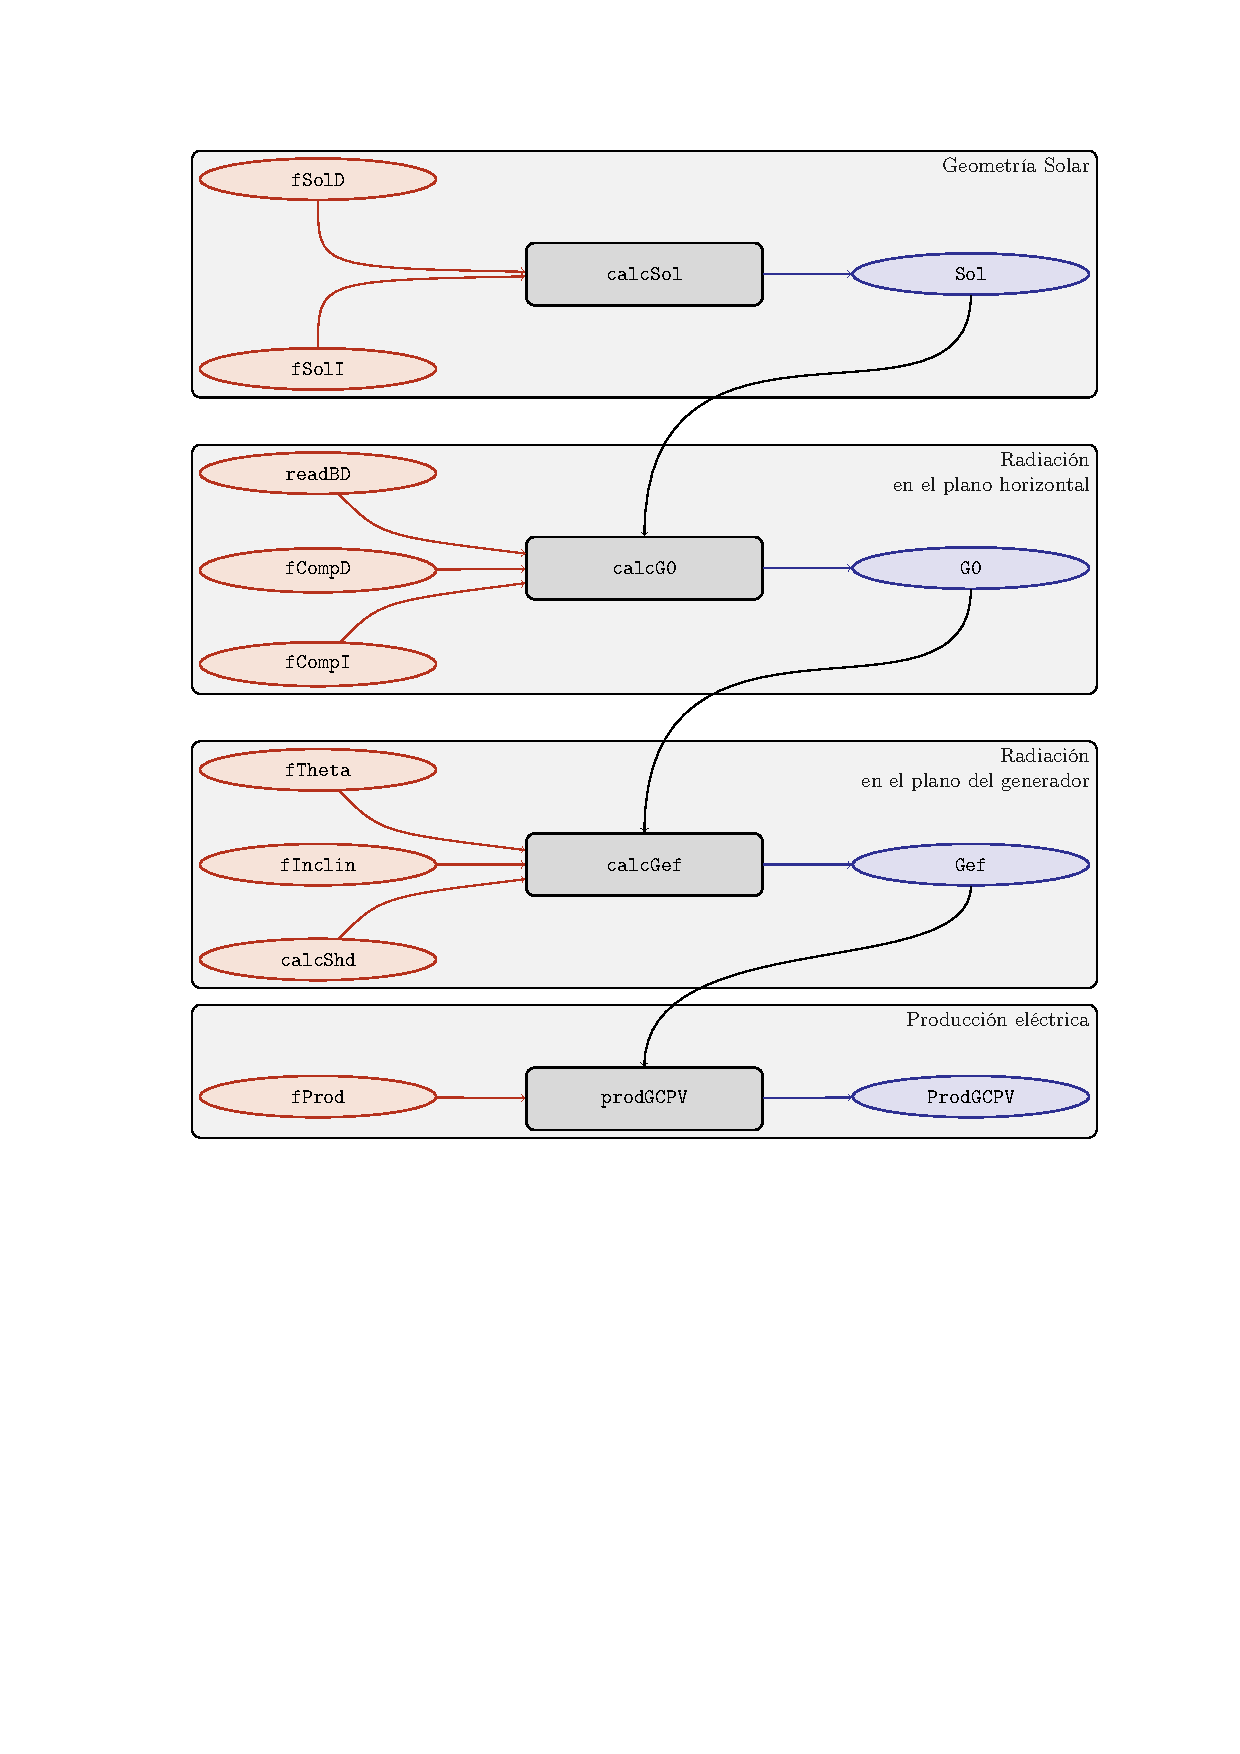
\includegraphics[keepaspectratio,width=0.8\textwidth,height=0.5\textheight]{figuras/procedure.pdf}
\caption{\label{fig:org9123200}Proceso de cálculo de las funciones de \texttt{solaR2}}
\end{figure}
A la hora de estimar la producción, el programa sigue los siguientes procesos:
\subsection{Geometría que definen la posición de la Tierra frente al Sol.}
\label{sec:orgbf15051}
\begin{enumerate}
\item Mediante la función fSolD, se calcula:
\begin{itemize}
\item El ángulo de declinación de la Tierra (\(\delta\)).
\item La corrección debida a la excentricidad de la elipse de la trayectoria terrestre alrededor del sol (\(\epsilon_0\)).
\item La ecuación del tiempo (\(EoT\)).
\item El ángulo del amanecer
\end{itemize}
\item Mediante la función fSolI, se calcula:
\begin{itemize}
\item La hora solar (\(\omega\)).
\item El momento del día en el que es de noche.
\item El ángulo zenital solar (\(\theta_{zs}\)).
\item El ángulo de altura solar (\(\gamma_s\)).
\item El ángulo azimutal solar (\(\psi_s\)).
\item La irradiancia extra-terrestre en el plano horizontal (\(B_0(0)\)).
\end{itemize}
\item El resultado de ambas funciones se juntan en un solo objeto de clase \texttt{Sol} mediante la función calcSol.
\end{enumerate}
\subsection{Radiación en el plano horizontal.}
\label{sec:orgb8651e2}
\begin{enumerate}
\item La información de irradiación en el plano horizontal (en todos sus componentes o, en su defecto, solo la global(\(G_d(0)\))) y temperatura viene dada en un objeto de clase \texttt{Meteo}.
\item Mediante la función fCompD, se calcula:
\begin{itemize}
\item La fracción de radiación difusa diaria (\(F_{Dd}\)).
\item El índice de claridad diario (\(K_{Td}\)).
\item Si solo se tienen datos de la componente global de irradición:
\begin{itemize}
\item La irradiación directa en el plano horizontal (\(B_d(0)\)).
\item La irradiación difusa en el plano horizontal (\(D_d(0)\)).
\end{itemize}
\end{itemize}
\item Mediante la función fCompI, se calcula:
\begin{itemize}
\item La fracción de radiación difusa (\(F_D\)).
\item El índice de claridad (\(K_T\)).
\item Si solo se tienen datos de la componenete global de irradiancia (\(G(0)\)):
\begin{itemize}
\item La irradiancia directa en el plano horizontal (\(B(0)\)).
\item La irradiancia difusa en el plano horizontal (\(D(0)\)).
\end{itemize}
\end{itemize}
\item El resultado de ambas funciones junto a medias mensuales y valores anuales se consolidan en un solo objeto de clase \texttt{G0} (que incluye los objetos \texttt{Sol} y \texttt{Meteo} de los que parte) mediante la función calcG0.
\end{enumerate}
\subsection{Radiación en el plano del generador.}
\label{sec:org32fd1d1}
\begin{enumerate}
\item La información de radiación puede venir dada en forma de un objeto de clase \texttt{Meteo} o un objeto de clase \texttt{G0} (ya que es este último el que se necesita para estimar la radiación en el plano del generador).
\item Mediante la función fTheta, se calcula:
\begin{itemize}
\item Ángulo de inclinación de la superficie del módulo (\(\beta\)).
\item Ángulo azimutal de la superficie del módulo (\(\alpha\) ).
\item Ángulo de incidencia de la irradiancia solar en la superficie del módulo (\(\theta_s\)).
\end{itemize}
\item Mediante la función fInclin, se calcula:
\begin{itemize}
\item La irradiancia extra-terrestre en la superficie inclinada (\(B_0(\beta, \alpha)\)).
\item La irradiancia directa normal (\(B(n)\)).
\item Las irradiancias global (\(G(\beta, \alpha)\)), directa (\(B(\beta, \alpha)\)), difusa (\(D(\beta, \alpha)\))(total, isotropica y anisotrópica) y del albedo (\(R(\beta, \alpha)\)) sobre una superficie inclinada.
\item Las irradiancias efectivas global (\(G_{ef}(\beta, \alpha)\)), directa (\(B_{ef}(\beta, \alpha)\)), difusa (\(D_{ef}(\beta, \alpha)\))(total, isotropica y anisotrópica) y del albedo (\(R_{ef}(\beta, \alpha)\)) sobre una superficie inclinada.
\item Los factores de pérdidas angulares para las componentes directa (\(FT\)), difusa (\(FT_D\)), y del albedo (\(FT_R\)).
\end{itemize}
\item Mediante la función calcShd, se puede calcular:
\begin{itemize}
\item La irradiancia e irradiación incluyendo sombras para seguidores a dos ejes y horizontales y paneles fijos mediante la función fSombra.
\end{itemize}
\item El resultado de estas funciones junto a medias mensuales y valores anuales se consolidan en un solo objeto de clase \texttt{Gef} (que incluye el objeto \texttt{G0} del que parte) mediante la función calcGef.
\end{enumerate}
\subsection{Producción eléctrica.}
\label{sec:org4a176a8}
\begin{enumerate}
\item Mediante la función fProd, se calcula:
\begin{itemize}
\item La potencia en corriente continua (\(P_{DC}\)).
\item La potencia en corriente alterna (\(P_{AC}\)).
\end{itemize}
\item Estos resultados, llevados a valores diarios, mensuales y anuales, se pueden convertir en valores de energía (\(E_{DC}\) y \(E_{AC}\)) y de productividad del sistema (\(Y_f\)), los cuales se consolidan en un solo objeto de clase \texttt{ProdGCPV} (que incluye el objeto \texttt{Gef} del que parte) mediante la función prodGCPV.
\end{enumerate}
